% fig_charge.tex -- Figure 4.1: capacitor as charge bucket
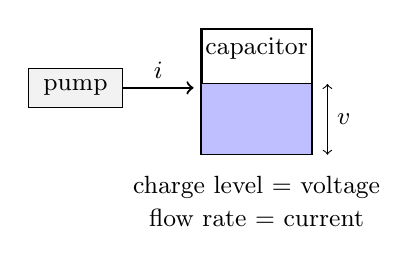
\begin{tikzpicture}
  % battery pumping charge
  \draw[fill=gray!10] (0,0) rectangle (1.2,0.5);
  \node at (0.6,0.25) {\small pump};
  \draw[->,thick] (1.2,0.25) -- (2.1,0.25);
  \node[above] at (1.65,0.25) {\small $i$};
  % bucket
  \draw[thick] (2.2,-0.6) -- (2.2,1.0) -- (3.6,1.0) -- (3.6,-0.6);
  \draw[fill=blue!25] (2.2,-0.6) rectangle (3.6,0.3);
  \draw[<->] (3.8,-0.6) -- (3.8,0.3) node[midway,right]{\small $v$};
  \node at (2.9,0.75) {\small capacitor};
  \node[below,align=center] at (2.9,-0.75) {\small charge level = voltage\\ \small flow rate = current};
\end{tikzpicture}
